\section{Small World Options}
\label{sec:theory}

% What are small world options
In Kleinberg's small-world network model, each node $u$ is given one
`long-range' edge to a node $v$, which was chosen with a probability
$P_r(u,v) \propto \|u-v\|^{-r}$, where $\|u-v\|$ denotes the distance
between $u$ and $v$ in the graph. Similarly for each state $s$, we add
a single `path option' to another state $s'$, where $s'$ is chosen with
probability $P_r(s,s') \propto \|s-s'\|^{-r}$. A path option $o_p(s,s')$
is an option with $\initset = \{s\}$, $\stopcond = \{s'\}$, and an
optimal policy to reach $s'$ for $\pi$. Intuitively, it is an option
that takes the agent from $s$ to $s'$. In practice, we may generate path
options only for a subset of $|S|$. Note that while $O(|S|)$ options are
created, only one additional option is available in any state, and thus
the decision-space for the agent is not significantly larger.

% What is the guarantee we give about them?
On an $r$-dimensional lattice, $\klein_r$, the distance from any node
$u$ to a target node $t$ is bounded by $\|u-t\|$, a quantity which is
locally computable. When given long-range edges distributed according to
$P_r$, Kleinberg showed that the greedy distributed algorithm
$\greedyalgo$ that chooses a neighbour $v$ closest to $t$ will reach $t$
with an expected time $O(\log(|V|)^2)$. This follows as a trivial
corollary of the following theorem,

\begin{theorem}
    \label{thm:small-world}
    %
    Let $f : V \to \Re$ be a function embedded on the graph
    $\graph(V,E)$, such that, $\kappa_1 \|u-v\| - c_1 \le \|f(u)
    - f(v)\| \le \kappa_2 \|u - v\| - c_2$, where $0 \le \kappa_1 \le
    \kappa_2$, and $0 \le c_2 \le \frac{c_1}{2}$. Let $M_f$ be the
    global maxima of $f$. Let \egreedyalgo be an $\epsilon$-greedy
    algorithm with respect to $f$, i.e.  an algorithm which chooses with
    probability $1-\epsilon$ to transit to the neighbouring state
    closest to $M_f$, i.e. $N(u) = \argmin_v \|f(v) - f(M_f)\|$.
    
    If $\graph(V,E)$ is $r$-dimensional lattice, and contains a long
    distance edge distributed $P_r$, then \egreedyalgo takes $O( (\log
    |V|)^2 )$ steps to reach $M_f$.
\end{theorem}
\begin{proof}
  The key insight of the proof is that with edges distributed according
  to $P_r$, there will always be edge within the neighbourhood of a node
  to an exponentially smaller neighbourhood of the target. Thus, the
  agent will only require to hop through $\log |V|$ `neighbourhoods'. By
  bounding the time spent in each neighbourhood to $\log |V|$, we arrive
  at the result. We refer the reader to
  \appendixref{sec:small-world-theory} for the complete proof.
\end{proof}

\begin{figure}[th]
    \centering
    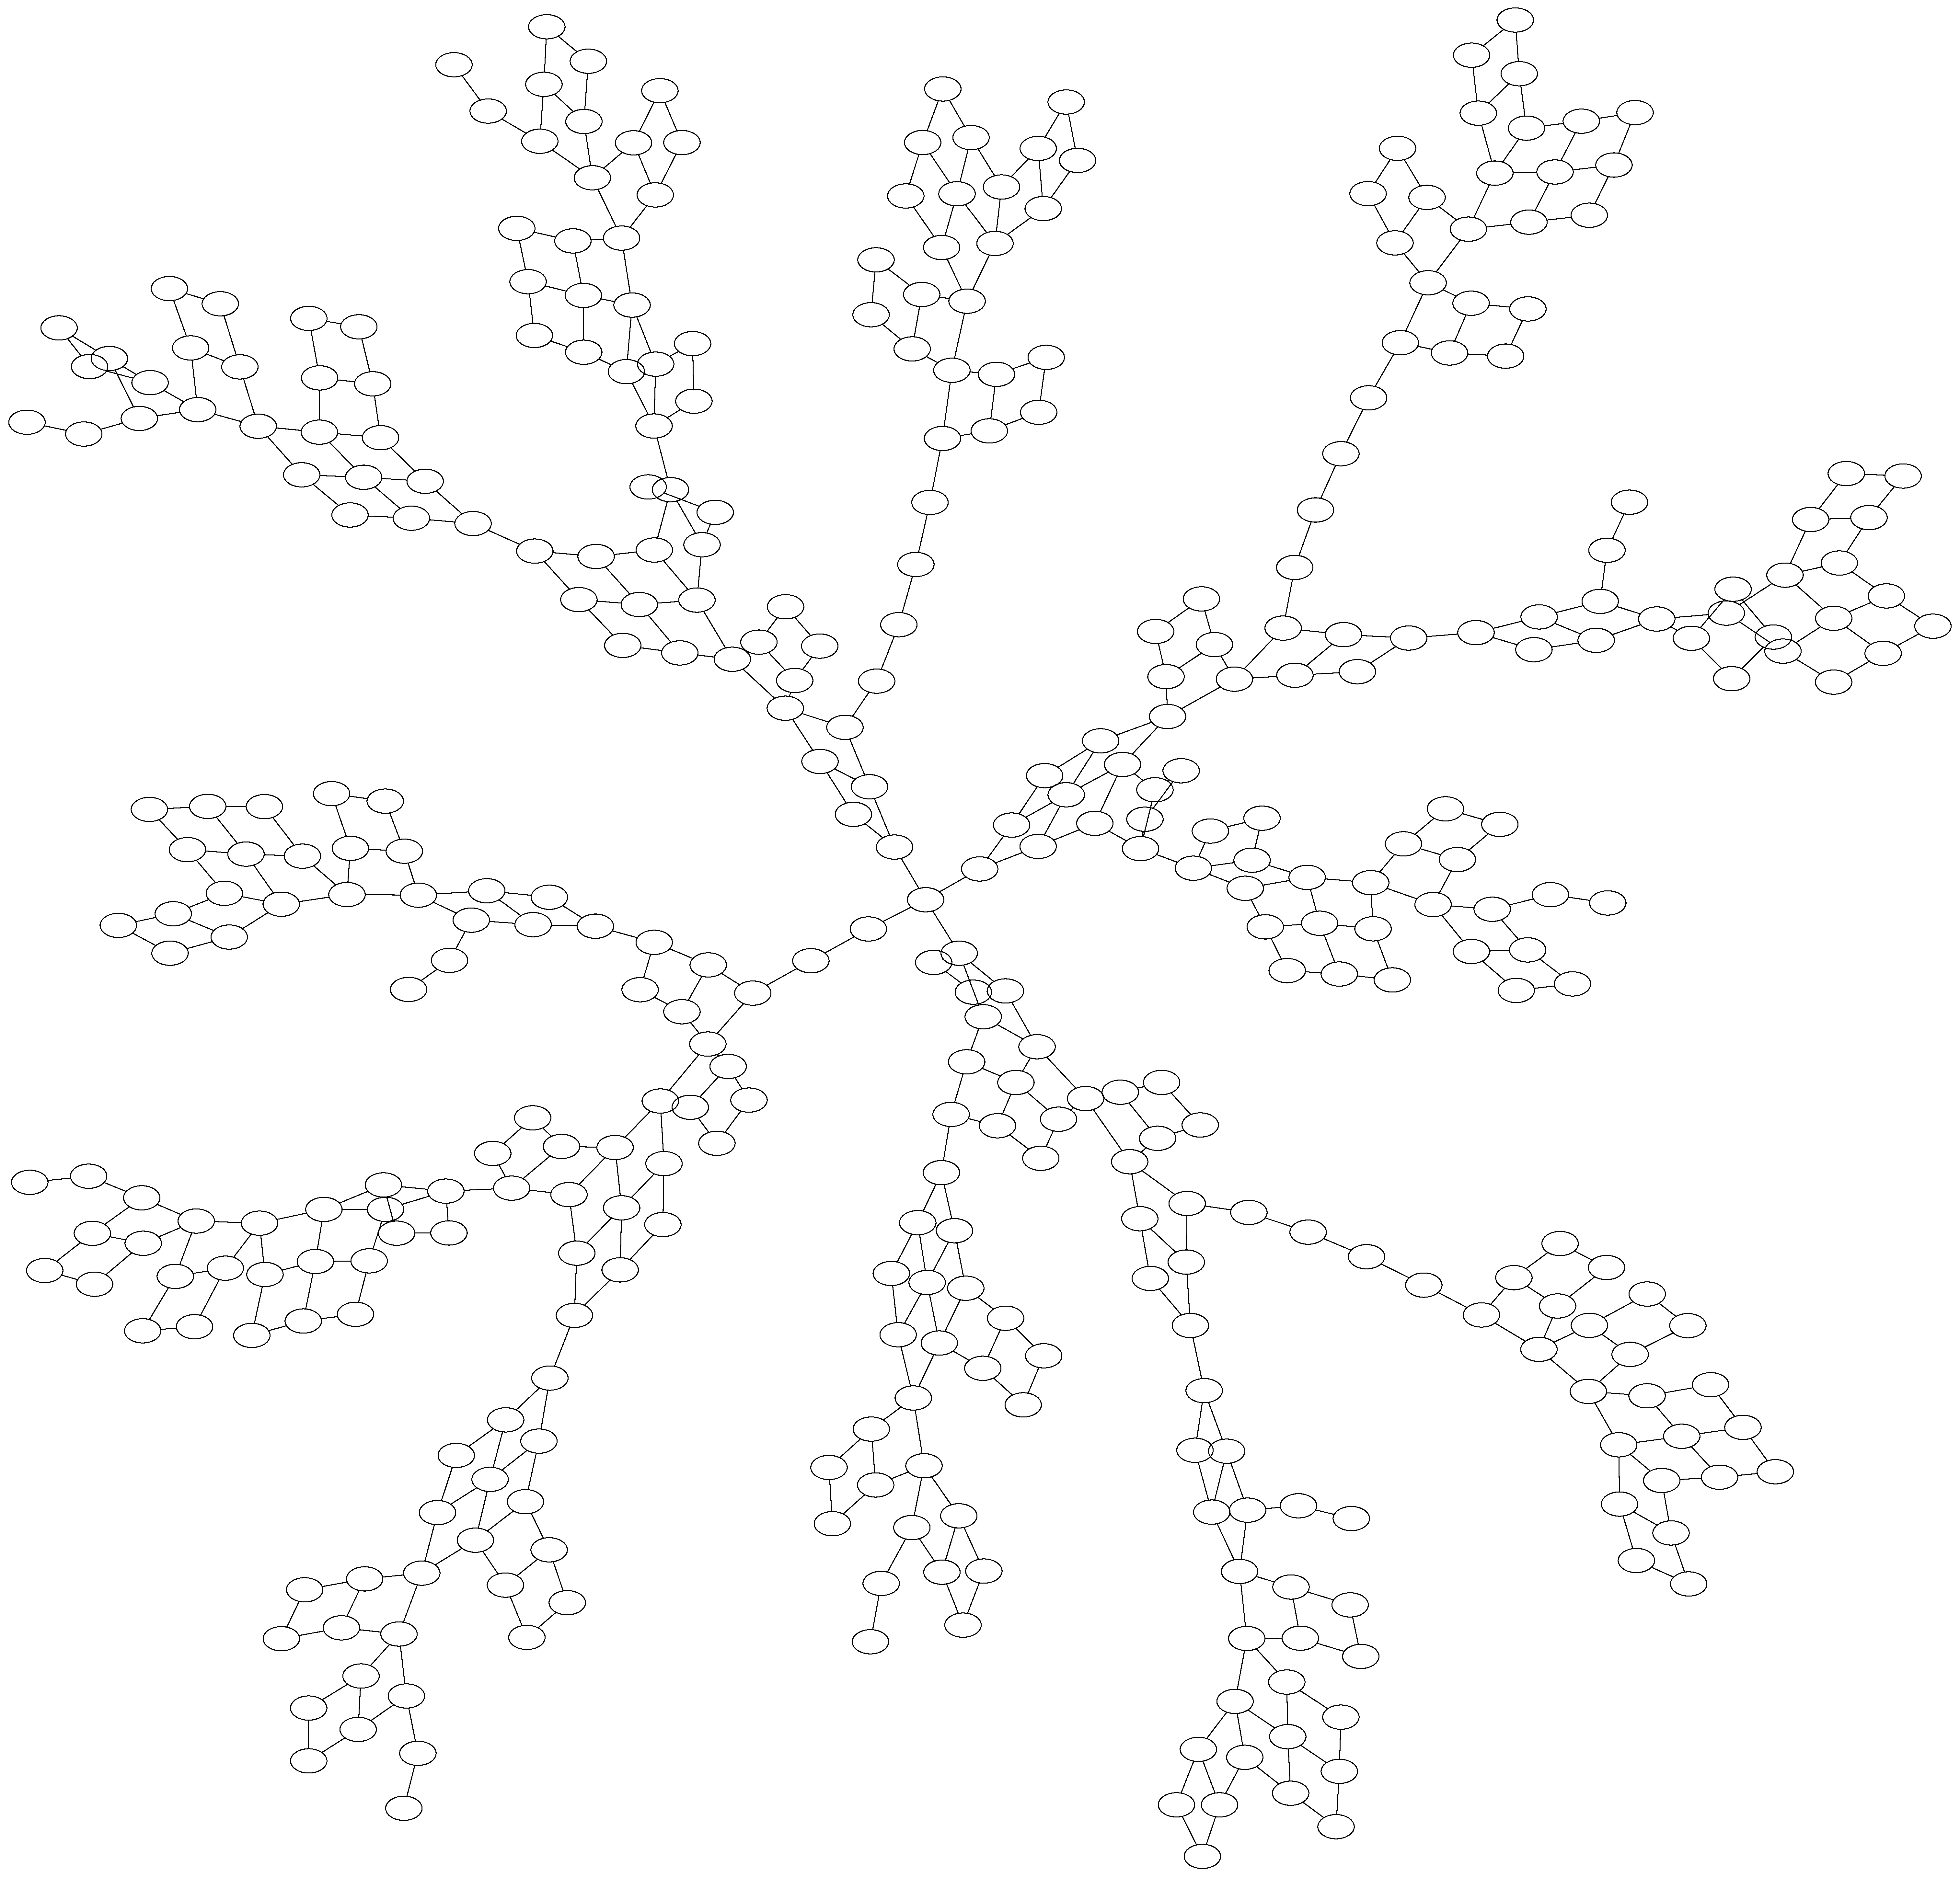
\includegraphics[height=2in]{figures/taxi1}
    \label{fig:taxi-graph}
    \caption{The State Space Graph for Taxi}
\end{figure}

% Graph-based
It is easy to construct a graph $\graph_{\mdp}$ out of the state-space
described by an MDP. The states $\states$ become the nodes of the graph,
and actions $\actions$ become the edges, with the transition
probabilities as weights. The edges can also be attributed with the
rewards described by $\rewards$. Options can be viewed to be paths along
the graph. As an example, the Taxi domain defined earlier translates to
the graph shown in \figref{fig:taxi-graph}.

Consider an MDP $\mdp_{\klein_r}$ with states connected in
a $r$-dimensional lattice, and noisy navigational actions between
states. We claim that using path options distributed according to $P_r$,
an $\epsilon$-greedy agent can reach a state of maximal value using
$O(\log(|S|)^2)$ options. Clearly, the value function $\Vf$ is a local
property of the state. Thus, if we can relate $\Vf$ to the distance from
the target state, we can apply \thmref{thm:small-world}.

\begin{definition}
    A {\em robust path option} $o(u,v)$, where $u,v \in \states$ is an
    option that takes the agent from $u$ to $v$ `robustly', in the
    sense that in each epoch, the agent moves closer to $v$ with a
    probability $1-\epsilon > \frac{1}{2}$. \footnote{This condition
    is equivalent to saying that the option takes the agent from $u$
    to $v$ in finite time, and hence is not particularly strong.}.
    Note that this $\epsilon$ includes any environmental effects as
    well.
\end{definition}

The following lemma shows that $\Vf$ satisfies the properties of a
embedded function required for \thmref{thm:small-world}. 

\begin{lemma}
    \label{lm:distance}
    Let $o(u,v)$ be the preferred option in state $u$, and let $\|u -
    v\|_V = |\log \Vf(v) - \log \Vf(u)|$. Then, 
    \begin{IEEEeqnarray*}{rCCCl}
        k_1 \|u - v\| - c_1 & \le & \|u - v\|_V & \le & k_2 \|u - v\|, 
    \end{IEEEeqnarray*}
    \noindent
    where $k_1 = \log \frac{1}{\gamma} $, $k_2 = \log
    \frac{1}{(1-\epsilon)\gamma}$, and $c_1 = \log
    \frac{1}{1-\gamma}$.
\end{lemma}
\begin{proof}
    For notational convenience, let $\epsilonm = 1 - \epsilon$. From the Bellman optimality condition, we get the value of $o(u,v)$ to be,
    \begin{eqnarray*}
        \Qf(u, o(u,v)) &=& \E_{l}[ \gamma^{l} \Vf(v) + \sum_{i=1}^{l} \gamma^{i-1} r_i ],
    \end{eqnarray*}
    \noindent
    where $l$ is the length of the option, and $r_i$ is the reward
    obtained in the $i$-th step of following the option. 
    
    If o(u,v) is the preferred option in state $u$, then $\Vf(u) =
    \Qf(u, o(u,v))$.  Using the property that $0 \le r_i \le 1$,
    \begin{IEEEeqnarray*}{rCCCl}
        \E_{l}[ \gamma^{l} \Vf(v) ] &\le& \Vf(u) &\le& \E_{l}[ \gamma^{l} \Vf(v) + \sum_{i=1}^{l} \gamma^{i-1}] \\
        \E_{l}[ \gamma^{l} ] \Vf(v) &\le& \Vf(u) &\le& \E_{l}[ \gamma^{l} ] \Vf(v) + \frac{1}{1 - \gamma}. \IEEEyesnumber \label{eq:v-bound}
    \end{IEEEeqnarray*}

    $\E_{l}$ is an expectation over the length of the option. Using
    the property that $o(u,v)$ is robust, we move closer to $v$ with
    probability $\epsilonm$; this is exactly the setting of the
    well-studied gambler's ruin problem, where the gambler begins with
    a budget of $\|u-v\|$, and wins with a probability of $\epsilon$.

    \begin{lemma}
        Consider the gambler's ruin problem where the gambler begins 
        with a budget of $m$, and has a winning probability of $q < \frac{1}{2}$
        (the dealer has a winning probability of $p=1-q$). Let $L$ be
        a random variable for the length of the game. Then, 
        \begin{eqnarray*}
            g_m(x) = \sum_{l=0}^{\infty} P(L = l) x^{l} &=& \frac{1}{\lambda_1^m( x ) + \lambda_2^m( x )},
        \end{eqnarray*}
        \noindent
        where $\lambda_1(x) = \frac{1 + \sqrt{1 - 4pq x^2}}{2px}$, and
        $\lambda_2(x) = \frac{1 - \sqrt{1 - 4pq x^2}}{2px}$.

        Further, when $x \le 1$,
        \begin{IEEEeqnarray*}{rCCCl}
            (px)^m  &\le&  g_m(x) &\le& x^m.
        \end{IEEEeqnarray*}
    \end{lemma}
    \begin{proof}
        For the first part. refer \cite{Feller1968}.

        The second part follows as a corollary, 
        \begin{IEEEeqnarray*}{rCCCl}
            \frac{1}{ (\lambda_1( x ) + \lambda_2( x ) )^{m} }  &\le&  g_m(x) &\le& \sum_{l=m}^{\infty} P(L = l) x^{l} \\
            \frac{1}{(\frac{2}{2px})^m}  &\le&  g_m(x) &\le& \sum_{l=m}^{\infty} P(L = l) x^{m} \\
            (px)^m  &\le&  g_m(x) &\le& x^m.
        \end{IEEEeqnarray*}
    \end{proof}

    In our situation, $p = 1 - \epsilon = \epsilonm > \frac{1}{2}$, $q = \epsilon$, and $m = \|u - v\|$.     
    \begin{IEEEeqnarray*}{rCCCl}
        (\epsilonm \gamma)^{\|u-v\|} &\le& \E_{l}[ \gamma^{l} ] &\le& (\gamma)^{\|u-v\|}.
    \end{IEEEeqnarray*}

    Returning to \eqnref{eq:v-bound},
    \begin{IEEEeqnarray*}{rCCCl}
        \E_{l}[ \gamma^{l} ] \Vf(v) &\le& \Vf(u) &\le& \E_{l}[ \gamma^{l} ] \Vf(v) + \frac{1}{1 - \gamma} \\
        (\epsilonm \gamma)^{\|u-v\|} \Vf(v) &\le& \Vf(u) &\le& \gamma^{\|u-v\|} \Vf(v) + \frac{1}{1 - \gamma} \\
        \|u-v\| \log \frac{1}{\gamma} - \log \frac{1}{1-\gamma} &\le& \|u - v\|_V &\le& \|u-v\| \log (\frac{1}{\epsilonm \gamma}).
    \end{IEEEeqnarray*}

\end{proof}

